% !TEX root = ../main.tex

\section{Test} \label{sec:test}

For this project, not many tests where performed. The tests where only for
smaller components as the structural breaks algorithm by design is random and
the outcome is not the same each time. The tests are only black box tests. 

Another reason for the lack of tests was simply the scope of the project. It is
not a very large project, and the amount of testable components is small. But a
few tests are performed and can serve as a proof of concept. 

\subsection{Components}

Tests were performed on the individual components to make sure they worked as
intended. This was both the case for custom data structures and other objects. 

For the range trees, a few tests were carried out to check that the queries
returned the correct values. This was useful for making sure the data
structure worked as intended.  

Other tests were also carried out for the objects like \texttt{Individual} and
\texttt{Genome} while they were being implemented. For the genome, it was
important that the break point indexes are in increasing order. 

\subsection{Running time} \label{sec:test-running-time}

For testing running times, a simple class \texttt{runTimeTimer} was made. It has
two methods \texttt{start()} and \texttt{stop()}. \texttt{start()} must be called
before the code chunk to be examined. \texttt{stop()} must be called just after.
The running time will appear in milliseconds in the console. 

\subsection{The algorithm} \label{sec:test-the-algorithm}

As mentioned above, the algorithm will not return the same result each time due
to the randomness. Thus, for testing the algorithm actually works, the result
was displayed either in the terminal or on the GUI, see
figure~\ref{fig:bp-locations}. For displaying in the
terminal, the fittest individual was printed. The GUI displays the fittest
individual in accordance with the fitness model. The "tests" were black box
tests with subjective evaluation. 

\begin{figure}[ht]
    \centering
    \begin{subfigure}[b]{.48\textwidth}
        \centering
        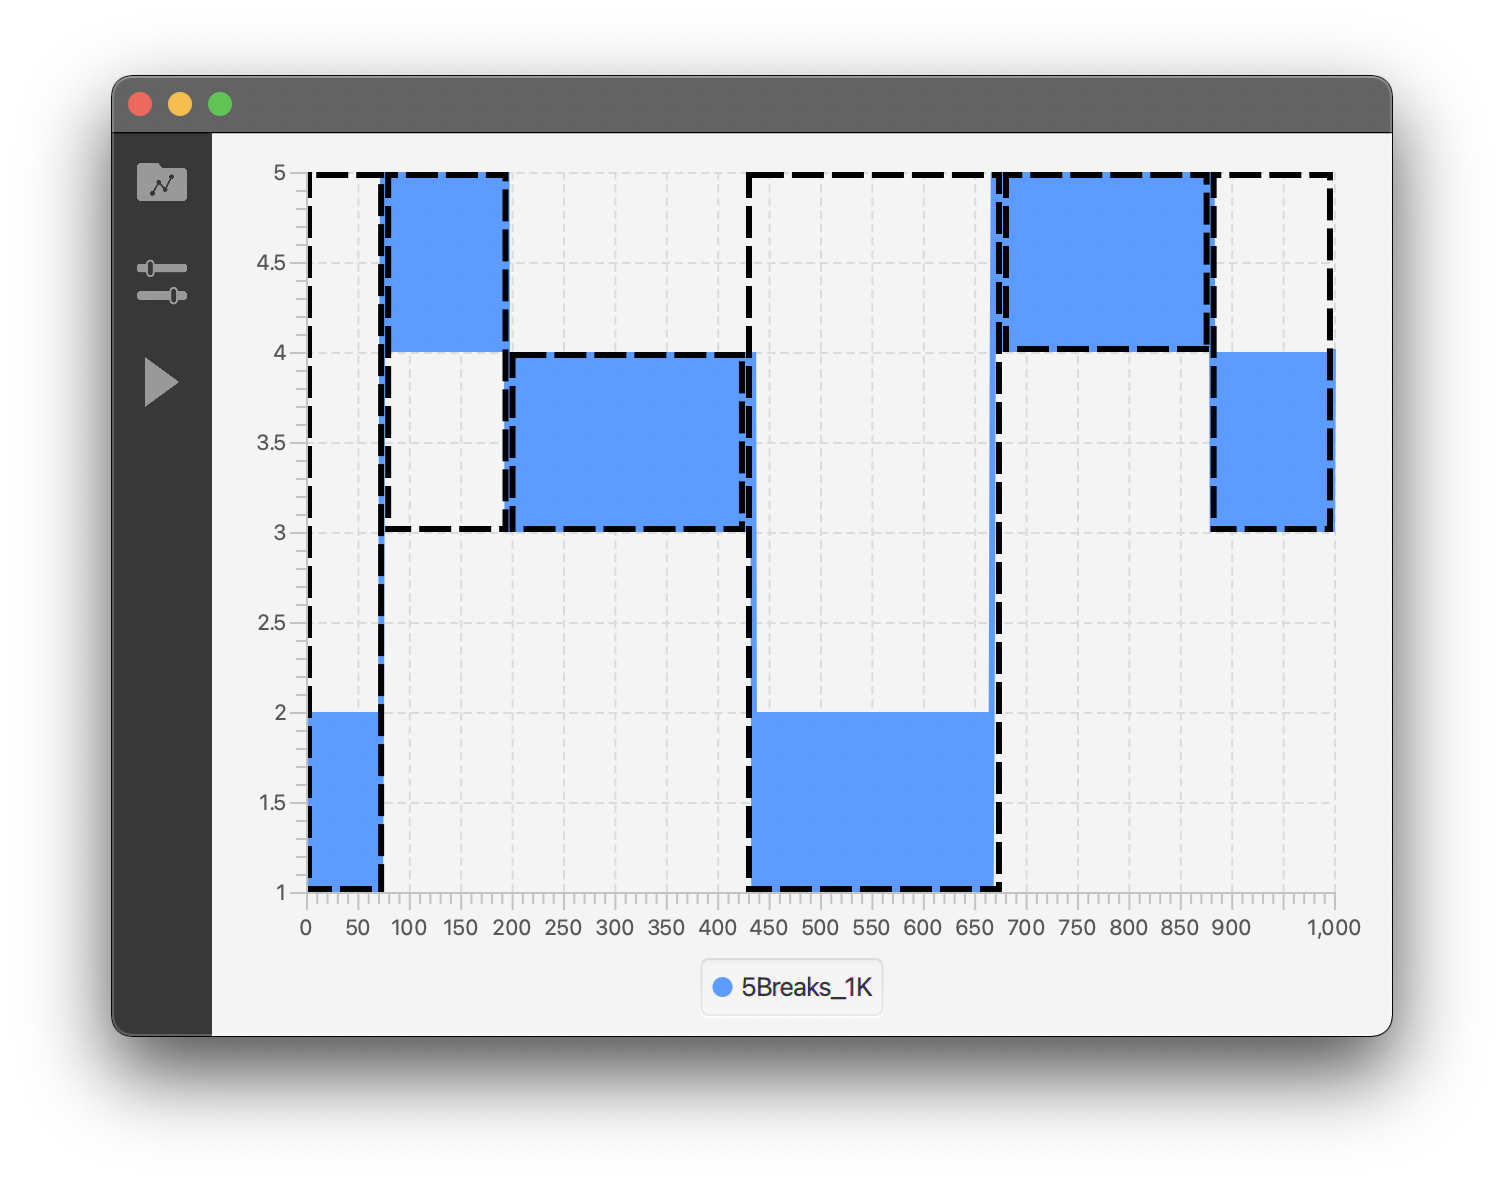
\includegraphics[width=\textwidth]{fig/bp-locations-gui.png}
        \caption{Algorithm output in GUI}
        \label{fig:bp-locations-gui}
    \end{subfigure}
    \hfill
    \begin{subfigure}[b]{.48\textwidth}
        \centering
        \raisebox{20mm}{%
            
\includegraphics[width=\textwidth]{fig/bp-locations-terminal.png}
        }
        \caption{Algorithm output in terminal}
        \label{fig:bp-locations-term}
    \end{subfigure}
    \caption{Displaying the output of the algorithm for testing. (Results from the same run)}
    \label{fig:bp-locations}
\end{figure}

In theory, some automatic tests could be set up. This could be a matter of
testing for fitness: Testing if the fitness of the fittest individual never
declines during the algorithm; testing if the fitness of the final fittest
individual is within a certain range of the optimal fitness for a given time
series. These seem somewhat abstract though and are therefor not implemented
during this project. 